\documentclass{article}
\usepackage{tikz}
\usetikzlibrary{arrows.meta,positioning}

\begin{document}
\section{Pipeline}
The data flows through three stages.

\begin{center}
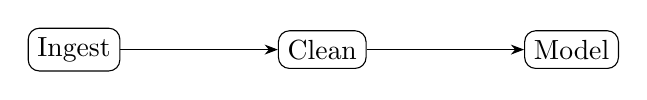
\begin{tikzpicture}[node distance=2cm, every node/.style={draw, rounded corners}]
  \node (a) {Ingest};
  \node (b) [right=of a] {Clean};
  \node (c) [right=of b] {Model};
  \draw[-Stealth] (a) -- (b);
  \draw[-Stealth] (b) -- (c);
\end{tikzpicture}
\end{center}

Each stage runs as a separate job.
\end{document}
